%lijst met inhoud in de marge
\input{../preamble}
\begin{document}

\section*{aantekeningen (uit bronnen van) EdX course}

idee:
Moeder Natuur berekent \par
Hefboom: gewogen gemiddelde \par
serie weertanden: optellen \par
parallelle weerstanden: reciprook optellen
lenzenformule
twee gewichten op een weegschaal

Maar er zijn meer regels. Voor quantum systemen kun je beter quantumregels gebruiken. Berekenen van chemische substanties


bronnen
Quantum Zoo \footnote{\url{https://math.nist.gov/quantum/zoo/}}
Quanttiki \footnote{\url{https://www.quantiki.org/wiki/teleportation-protocol}}

bij de vragen: parser geeft het geinterpreteerde getal weer.
Hiervoor is een submit knop nodig
Die heb je ook nodig voor een meermerkeuzevraag
Understanding chemistry
Zuurstof met twee streepjes

De covalente binding Uitleg in Absolutely small

The focus in QM is shifting from $$\frac{i}{\hbar}\frac{d\Psi}{dt}= H \Psi$$
to
 
\vspace{0.5cm}
\Qcircuit @C=1em @R=2em {
\ustick{\ket{0}}& \qw & \targ & \qw & \qw & \ustick{\ket{}}\\
\ustick{\ket{0}} & \gate{H} & \ctrl{-1} & \qw & \qw & \ustick{}
}
\vspace{0.5cm}

information

Nice: Solving a maze animation

Challenges for society
\begin{itemize}[nosep]
\item spoiling enery
\item waisint materials
\item climate is changing too fast
\item need for medicine
\item ..
\end{itemize}

\begin{itemize}[nosep]
\item electrical cables without loss of energy
\item Drug development (Quantum Chemistry)
\item Predicting material properties for electronics, energy storage
\item machine learning
\item optimization in robotics
\item handling big data for sequencing genomics
\item airplane desing
\item ..
\end{itemize}

photosynthesis pathway antenna chlorophyll: extreme fast solving of labyrinth

film Lieven van der siepen:
Twee mensen lopen in schadusspel en botsen, of lopen langs elkaar .
(plato's grot, superpositie)

film how to iunderstand superposition
Stel dat electronen twee eigenschappen hebben, kleur en hardheid

kleur: [B,W]
hardheid: [H,S]
(hmm zacht en zwart zelfde letter)
twee apparaten: een om kleur te sorteren, en een om hardheid te sorteren
(eigenlijk spin in twee verschillende richtingen,

\begin{center}  %DE manier om figuur te ontfloaten.
\leavevmode
%needs \usetikzlibrary{decorations.markings} in preambule
\tikzset{middlearrow/.style={
        decoration={markings,
            mark= at position 0.5 with {\arrow{#1}} ,
        },
        postaction={decorate}
    }
}

\begin{tikzpicture}[scale=.5]
%\def\x{0} 
\begin{scope}[xshift=0 cm]
\draw [fill=red!20] (0,0) rectangle  (3,3);
\draw (-1, 1.5) node[anchor=south] {800 el} -- (1.5,1.5);
\draw [middlearrow={latex}] (1.5,1.5) -- (3.5,1.5) node[anchor=north,xshift=1em] {B 50\%};
\draw [middlearrow={latex}] (1.5,1.5) -- (1.5,3.5) node[above] {W 50\%};
\node at (1.5,-.5) {colorbox};
\end{scope}

\begin{scope}[xshift=7 cm]
\draw [fill=gray!20] (0,0) rectangle  (3,3);
\draw (-1, 1.5) node[anchor=south] {400 el} -- (1.5,1.5);
\draw [middlearrow={latex}] (1.5,1.5) -- (3.5,1.5) node[anchor=north,xshift=1em] {H 200};
\draw [middlearrow={latex}] (1.5,1.5) -- (1.5,3.5) node[above] {S 200};
\node at (1.5,-.5) {hardnessbox};
\end{scope}

\end{tikzpicture}

\captionof{figure}{experiment 1  \label{fig:exp1}}
\end{center}

\begin{center}  %DE manier om figuur te ontfloaten.
\leavevmode
%needs \usetikzlibrary{decorations.markings} in preambule
\tikzset{middlearrow/.style={
        decoration={markings,
            mark= at position 0.5 with {\arrow{#1}} ,
        },
        postaction={decorate}
    }
}

\begin{tikzpicture}[scale=.5]
\begin{scope}[xshift=0 cm]
\draw [fill=gray!20] (0,0) rectangle  (3,3);
\draw (-1, 1.5) node[anchor=south] {400 el} -- (1.5,1.5);
\draw [middlearrow={latex}] (1.5,1.5) -- (3.5,1.5) node[anchor=north,xshift=1em] {H 200};
\draw [middlearrow={latex}] (1.5,1.5) -- (1.5,3.5) node[above] {S 200};
\node at (1.5,-.5) {hardnessbox};
\end{scope}

\begin{scope}[xshift=7 cm]
\draw [fill=red!20] (0,0) rectangle  (3,3);
\draw (-1, 1.5) node[anchor=south] {800 el} -- (1.5,1.5);
\draw [middlearrow={latex}] (1.5,1.5) -- (3.5,1.5) node[anchor=north,xshift=1em] {B 50\%};
\draw [middlearrow={latex}] (1.5,1.5) -- (1.5,3.5) node[above] {W 50\%};
\node at (1.5,-.5) {colorbox};
\end{scope}

\end{tikzpicture}

\captionof{figure}{experiment 2  \label{fig:exp2}}
\end{center}

\begin{center}  %DE manier om figuur te ontfloaten.
\leavevmode
%needs \usetikzlibrary{decorations.markings} in preambule
\tikzset{middlearrow/.style={
        decoration={markings,
            mark= at position 0.5 with {\arrow{#1}} ,
        },
        postaction={decorate}
    }
}

\begin{tikzpicture}[scale=.5]
\begin{scope}[xshift=0 cm]
\draw [fill=gray!20] (0,0) rectangle  (3,3);
\draw (-1, 1.5) node[anchor=south] {400 el} -- (1.5,1.5);
\draw [middlearrow={latex}] (1.5,1.5) -- (3.5,1.5) node[anchor=north,xshift=1em] {H 200};
\draw [middlearrow={latex}] (1.5,1.5) -- (1.5,3.5) node[above] {S 200};
\node at (1.5,-.5) {hardnessbox};
\end{scope}

\begin{scope}[xshift=7 cm]
\draw [fill=red!20] (0,0) rectangle  (3,3);
\draw (-1, 1.5) node[anchor=south] {800 el} -- (1.5,1.5);
\draw (1.2, 3.2) -- (1.8, 3.8);
\draw (3.2, 1.8) -- (3.8, 1.2);
\draw (3.2, 3.8) -- (3.8, 3.2);
\draw [dashed] (1.5,3.5)--(3.5,3.5) -- (3.5,1.5);
\draw [middlearrow={latex}] (1.5,1.5) -- (3.5,1.5) node[anchor=north,xshift=1em] {B 50\%};
\draw [middlearrow={latex}] (1.5,1.5) -- (1.5,3.5) node[above] {W 50\%};
\node at (1.5,-.5) {colorbox};
\end{scope}

\begin{scope}[xshift=14 cm]
\draw [fill=red!20] (0,0) rectangle  (3,3);
\draw (-1, 1.5) node[anchor=south] {800 el} -- (1.5,1.5);
\draw [middlearrow={latex}] (1.5,1.5) -- (3.5,1.5) node[anchor=north,xshift=1em] {B 50\%};
\draw [middlearrow={latex}] (1.5,1.5) -- (1.5,3.5) node[above] {W 50\%};
\node at (1.5,-.5) {colorbox};
\end{scope}

\end{tikzpicture}

\captionof{figure}{experiment 2  \label{fig:exp2}}
\end{center}


\subsection*{module 2}
trage video: 
superposition interference entanglement
cloning is not possible
error correction not simple but can be done

Divicencio
\begin{itemize}[nosep]

\item QC must be scalable
\item Qbits must be initiable
\item good qbits are needed, long coherence
\item have a universal set of quantum gates
\item you can measere them
\end{itemize}
video
high-level languare to
compiler
error correction
converted into quantum instructions
converted into physical signals (pulsees) to control and operate physical qubits
time constraint
synchonicity is a challenge

\subsubsection*{video what is q internet?}
technologies not available in classic internet
\begin{itemize}
\item secure communication
\item secure identification
\item position verification
\item secure dedicated computing
\item ...
\end{itemize}
\textbf{end node} are qcompters small ones, less than 10 qb, mosly 1 qb is enough
power of entanglement
incontrast on a qc we always need more qubits than can besimulated on a classical computer in order to do something new and interesting ??

\textbf{switches}
\textbf{repeaters}
\textbf{traffic control}

why powerful?
secure - not qubits cannot copied

entangelment
maximum coordination (=maximum correlation??)
only two qubits can be maximally entangled

\subsection*{module 3}
classic factoring goes with $2^n$ 
quantum factroing $N^3$
-hard to build
-need large nr of qubits to factor: a number of 2000 bitswill take 10000 qubits minimum
Redundancy needed for erroro correction vcan be factor of 1000-10000
So for now we are safe, but in 10-20 yrs other encryption systems are rerquitred


\subsubsection*{video encryption}
classic: shared key
One Time Pad
The message and key have the same length
Message and key are bitwise multiplied modulo 2
msg 0110
key 1010
enc 1100
if key==message send 0 else send 1
Bob can reverses the operation

msg ....
key 1010
enc 1100

Eve cannot decrypt the message if she has no info on the key


Sannon proved that to be totally secure, you need a key just as long as the message
A BW image 64x64=4096 bits info would require a 4096 bit key

in practice keys are much shorter

The number of key is limited. Easy proof (??)




A little variation of an example taken from the PGF documentation (Section 83 Repeating Things: The Foreach Statement, page 912 for version 3.0):


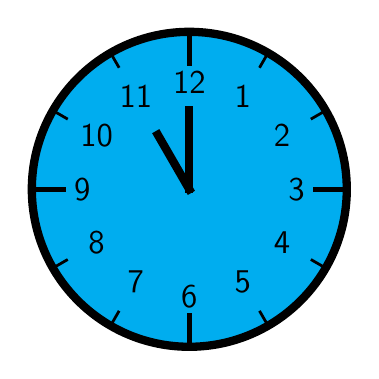
\begin{tikzpicture}[line cap=rect,line width=3pt]
\filldraw [fill=cyan] (0,0) circle [radius=2cm];
\foreach \angle [count=\xi] in {60,30,...,-270}
{
  \draw[line width=1pt] (\angle:1.8cm) -- (\angle:2cm);
  \node[font=\large] at (\angle:1.36cm) {\textsf{\xi}};
}
\foreach \angle in {0,90,180,270}
  \draw[line width=2pt] (\angle:1.6cm) -- (\angle:2cm);
\draw (0,0) -- (120:0.8cm);
\draw (0,0) -- (90:1cm);
\end{tikzpicture}
 
regels klok liegt niet (6 of 12) en (3 of 9).

Korte filmpjes 
-collapse in superposition (ps duidelijk na spel met klok) 

bit flip uitleg bitflip / sign flip is me onduidelijk

iig computational basis (6,12), Hadamard basis (3,9)
scenarios's met Alice, Bob, Eve
niet moeilijk.

\subsubsection*{module3, Learn more}

learn more encryptie methoden 
\textbf{RSA} \url{http://doctrina.org/How-RSA-Works-With-Examples.html} lastiger. 
meer voorbeelden bij multiplicatieve inverse nodig.

eulers\'s totient

shor's algorithm (wikipedia pagina) veel te lastig

\textbf{caesar's cipher} te simpel

\textbf{enigma machine} interessant maar off topic?

\textbf{braket} wikipaedia artikel overstijgt vwo niveau

\textbf{BB84} Bennett and Brassard 1984 \url{https://www.youtube.com/watch?v=UVzRbU6y7Ks&feature=youtu.be} zie ook teoelichting bij video.

volgt logischerwijs op spel met de klok

uit \url{https://www.youtube.com/watch?v=7SMcf1MdOaQ}:

\begin{table}[!htbp]//table op zijn plek houden
\centering
\begin{tabular}{
>{\columncolor[HTML]{FFFC9E}}l 
>{\columncolor[HTML]{67FD9A}}l 
>{\columncolor[HTML]{FD6864}}l 
>{\columncolor[HTML]{67FD9A}}l 
>{\columncolor[HTML]{FD6864}}l 
>{\columncolor[HTML]{FE0000}}l 
>{\columncolor[HTML]{67FD9A}}l 
>{\columncolor[HTML]{67FD9A}}l 
>{\columncolor[HTML]{FD6864}}l }
Alice's bit value    & 1 & 0 & 0 & 1 & 0 & 1 & 1 & 1  \\ 
Alice's sending mode & + & + & + & X & X & + & + & +  \\ 
Bob's receiving mode & + & + & X & + & + & + & + & X  \\ 
Bob's result         & 1 & 0 & 0 & 0 & 0 & 1 & 1 & 0  \\ 
Same mode?           & Y & N & Y & N & N & Y & Y & N  \\ 
Shared secret key    & 1 &   & 0 &   &   & 1 & 1 &    \\ 
\end{tabular}
\caption{BB-84}
\label{BB84}
\end{table}




\end{document}